% Appendix Template

\chapter{Results of experiment 2.6} % Main appendix title

\label{Appendix2-6} % Change X to a consecutive letter; for referencing this appendix elsewhere, use \ref{AppendixX}

\begin{figure}[th]
\centering
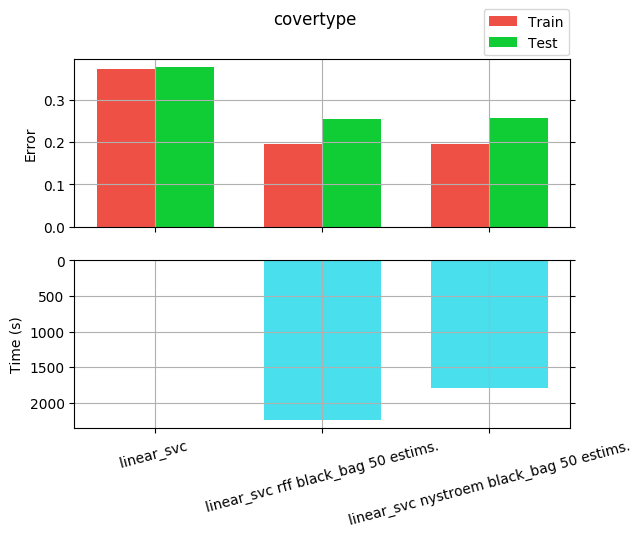
\includegraphics[scale=\imgscale]{Figures/2_6/covertype}
\decoRule
\caption[2.6 covertype]{Linear-SVM with Black Bag model}
\label{fig:2_6_covertype}
\end{figure}

\begin{figure}[th]
\centering
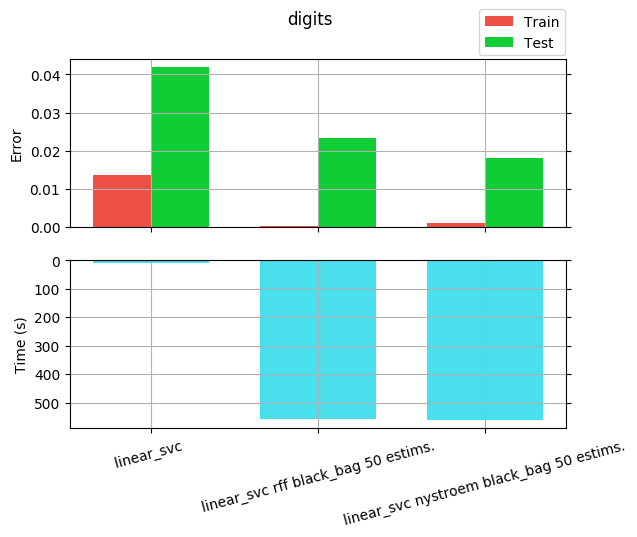
\includegraphics[scale=\imgscale]{Figures/2_6/digits}
\decoRule
\caption[2.6 digits]{Linear-SVM with Black Bag model}
\label{fig:2_6_digits}
\end{figure}

\begin{figure}[th]
\centering
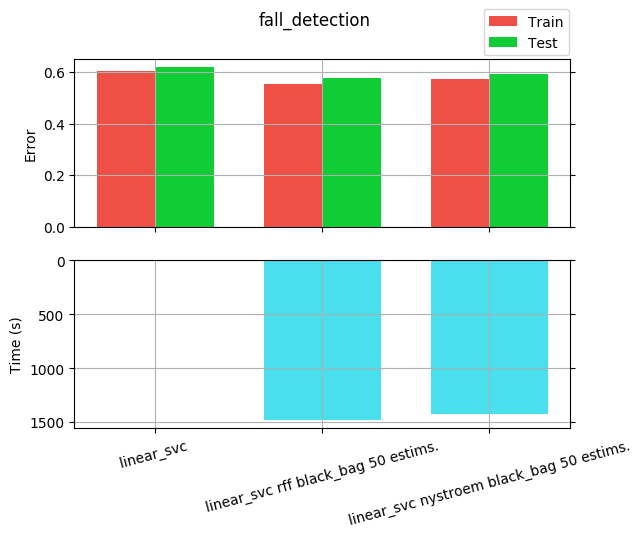
\includegraphics[scale=\imgscale]{Figures/2_6/fall_detection}
\decoRule
\caption[2.6 fall\tu detection]{Linear-SVM with Black Bag model}
\label{fig:2_6_fall_detection}
\end{figure}

\begin{figure}[th]
\centering
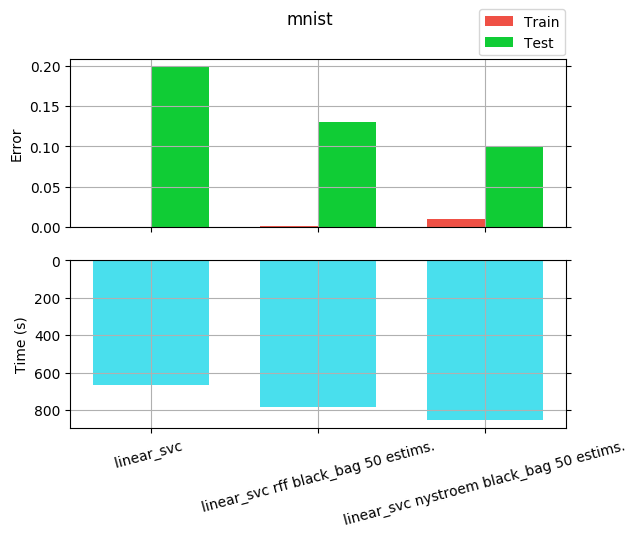
\includegraphics[scale=\imgscale]{Figures/2_6/mnist}
\decoRule
\caption[2.6 mnist]{Linear-SVM with Black Bag model}
\label{fig:2_6_mnist}
\end{figure}

\begin{figure}[th]
\centering
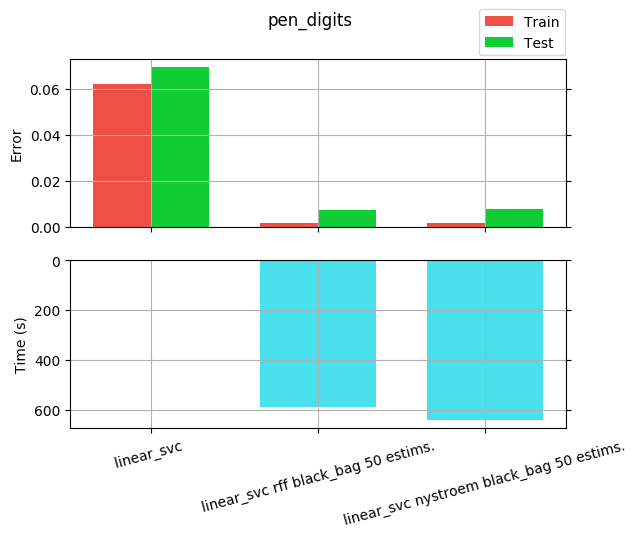
\includegraphics[scale=\imgscale]{Figures/2_6/pen_digits}
\decoRule
\caption[2.6 pen\tu digits]{Linear-SVM with Black Bag model}
\label{fig:2_6_pen_digits}
\end{figure}

\begin{figure}[th]
\centering
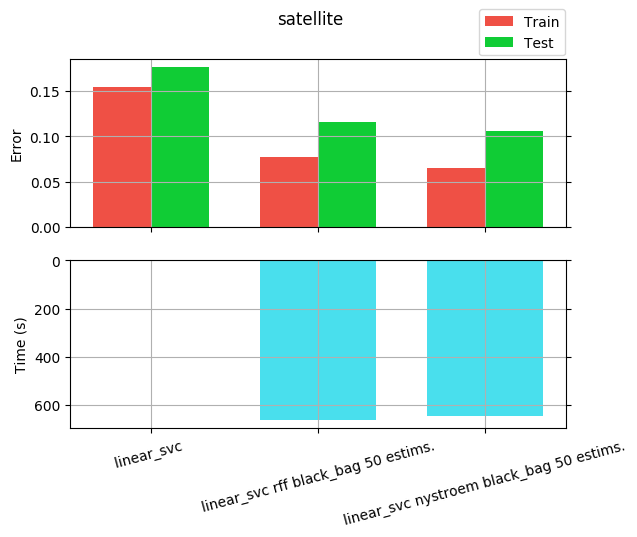
\includegraphics[scale=\imgscale]{Figures/2_6/satellite}
\decoRule
\caption[2.6 satellite]{Linear-SVM with Black Bag model}
\label{fig:2_6_satellite}
\end{figure}

\begin{figure}[th]
\centering
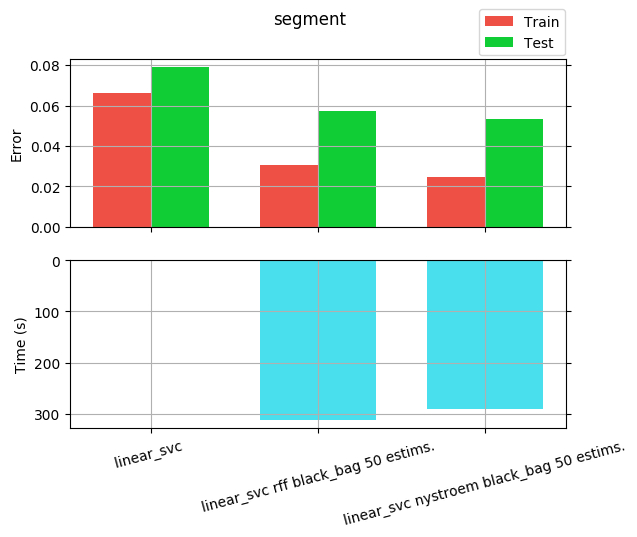
\includegraphics[scale=\imgscale]{Figures/2_6/segment}
\decoRule
\caption[2.6 segment]{Linear-SVM with Black Bag model}
\label{fig:2_6_segment}
\end{figure}

\begin{figure}[th]
\centering
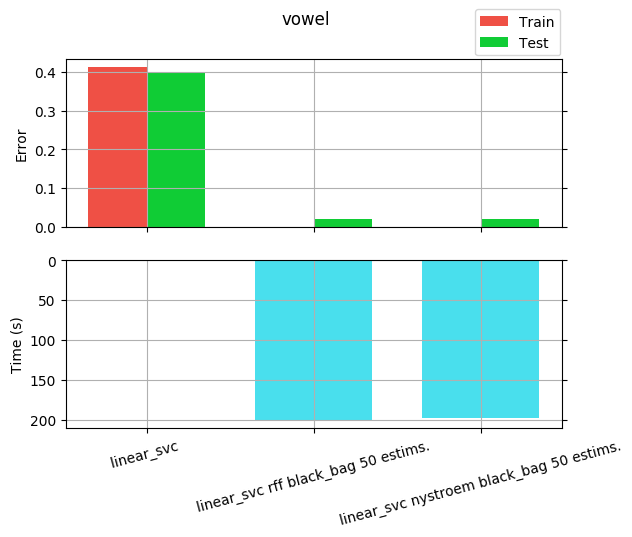
\includegraphics[scale=\imgscale]{Figures/2_6/vowel}
\decoRule
\caption[2.6 vowel]{Linear-SVM with Black Bag model}
\label{fig:vowel}
\end{figure}
